\documentclass{article}
\usepackage{multicol}
\usepackage{geometry}
\usepackage{blindtext}
\usepackage [autostyle, english = american]{csquotes}
\MakeOuterQuote{"}
\usepackage[sort, numbers]{natbib}
\usepackage{graphicx}
%\renewcommand{\familydefault}{\sfdefault}
%\usepackage{helvet}
\setlength{\columnsep}{1cm}
%\setlength{\columnseprule}{0.4pt}
\setlength{\footskip}{20pt}
\usepackage{fancyhdr}
\usepackage{hyperref}
\fancyhf{}
\fancyhead[C]{TransGlobalHealth $\bullet$ PhD Proposal $\bullet$ Joe Brew}
\fancyfoot[C]{  $\bullet$ joebrew@gmail.com $\bullet$  }
\renewcommand\headrulewidth{1pt}

\pagestyle{fancy}



\usepackage{Sweave}
\begin{document}
\Sconcordance{concordance:protocol.tex:protocol.Rnw:%
1 24 1 1 0 36 1 1 65 1 2 139 1}


\newgeometry{margin=2.5cm}



\begin{center}

\rule{\textwidth}{1.6pt}\vspace*{-\baselineskip}\vspace*{2pt} % Thick horizontal line
\rule{\textwidth}{0.4pt}\\[\baselineskip] % Thin horizontal line


\begin{LARGE}
\scshape{identifying opportunities: measuring the economic impact of malaria elimination in mozambique}
\end{LARGE}


\rule{\textwidth}{0.4pt}\vspace*{-\baselineskip}\vspace{3.2pt} % Thin horizontal line
\rule{\textwidth}{1.6pt}\\[\baselineskip] % Thick horizontal line

\begin{large}
Proposal for project 2: Foreign investments to finance malaria elimination: evidence from the south of Mozambique
\end{large}

\vspace{5mm}

\begin{Large}
Joe Brew
\end{Large}
\vspace{3mm}

\begin{large}
Erasmus Mundus, TransGlobalHealth PhD Proposal 
\end{large}

\vspace{10mm}
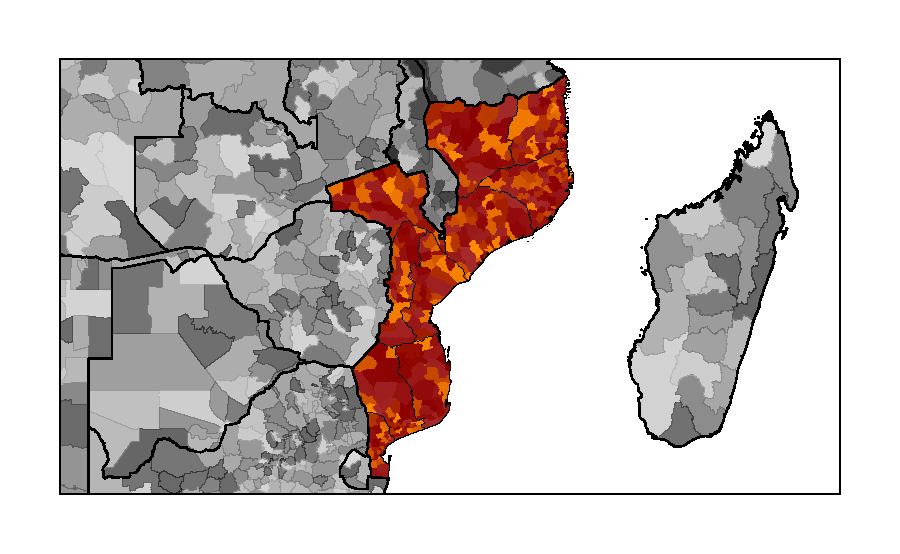
\includegraphics{protocol-001}

\vspace{5mm}


\subsection*{Project summary}

\end{center}



\noindent \emph{The elimination of malaria in Mozambique will require foreign capital.  The purpose of this project is to inform guide the flow of that capital to interventions, projects, business opportunities and areas which stand to gain the most from eradication, both in terms of economic and health improvements.  By (1) quantifying the burden of malaria across spatial and sociodegraphic lines, (2) modeling the impact of certain kinds of investments on the economy and health and (3) building a public "toolkit" to make sure that high-quality data are readily available to potential investors, this project seeks to facilitate the partnerships and collaborations necessary for the eradication of malaria.   } 


\newpage

\begin{multicols}{2}
\setkeys{Gin}{width=0.5\textwidth}



\noindent \textbf{Project:}\\ Identifying opportunities:\\ measuring the economic impact of malaria elimination in mozambique \\

\noindent \textbf{Investigator:} \\ Joe Brew, MPH, MA (applicant) 

\subsection*{General information} \\
The elimination of malaria from Mozambique is not an obstacle to be surmounted, but rather an opportunity to be seized.  The eradication of this disease will save countless lives, unleash the human potential of Mozambicans, and help to facilitate the country's fuller participation in the international economy.}

Elimination of malaria will require collaboration between large foreign funding sources, policy makers, and local public health practitioners.  The nature of this partnership, however, does not need to be based on aid; in fact, sustainable solutions will require that incentives and incentives be clearly measured, so as to attract foreign investment.  With good data, and a comprehensive presentation of those data, a symbiotic solution to Mozambique's malaria endemic can be achieved.  

Since the benefits of malaria eradication will traverse the health, education and industry sectors of the Mozambican economy, so to does the project seek to address eradication's economic impact across these lines.  By using standardized measurement tools and comparative observational analysis methods, eradication-related investment opportunities can be quantified in a way that will guide foreign investment for the mutual benefit of the investor, the people of Mozambique and the scientific and global health communities at large. 


\subsection*{Research questions:} What is the current economic burden of malaria in Mozambique?  Who are the current principle stakeholders in eradication, and what is \emph{their} prognosis on the campaign's sustainability?  Which sectors of the economy stand to gain most from eradication?  Which investment opportunities are likely to result in the greatest health and economic gains?

\subsection*{Study objectives}
The objectives of this project are three-fold: 
\begin{enumerate}
\item \textbf{Diagnosis:} Identify the current economic burden of malaria in mozambique across economic sectors, regions, time and sociodemographic groups.
\item \textbf{Prognosis:} Evaluate, model and compare projected intervention outcomes (quantifying uncertainty) both in terms of economic and health gains.
\item \textbf{Treatment:} Translate knowledge into action by building data "toolkits" and investment guides, fostering public-privatge partnerships, outlining best practices for eradication, and incorporating a strong evaluation component (for the post-project period) so that the global health, scientific and business communities can learn from the experience. 
\end{enumerate}


\subsection*{Study Design}
\noindent \textbf{Design:} Mixed methods (observational economic analysis, qualitative focus group interviews, probabilistic sensitivity analysis and Monte Carlo simulations). \\


\subsection*{Methodology}

\noindent \textbf{Phase 1:} For the "prognosis" phase of the project, I will conduct (a) a literature review of malaria-related economic evaluations, (b) a meta-analysis of the economic returns on malaria interventions in East Africa, and (c) a series of qualitative focus groups involving principal actors and stakeholders from both representative Mozambican political, economic and social groups, as well as potential international investment groups. The latter will take place only following approval from the appropriate ethical committees, institutional review boards, and governmental agencies. \\

\noindent \textbf{Phase 2:} For the "diagnosis" phase of the project, I will design, distribute, collect and analyze a large survey detailing labor market and social activity, as well as clinical history, among a representative cross-section of Mozambicans.  This will allow for a clear assessment of how malaria impacts economic activity and attitudes.  In the analysis, I will simulate (using established methods from the field of health economics\footnote{The methods will depend, to some extent, on the kind and quality of data available.  That said, my intention is to use stoachistic modeling to quantify both the likelihood and uncertainty of moving from different economic productivity "states" as a function of a region's or an individual's likelihood of malaria infection.  Hidden Markov models, such as Baum-Welch's method, as well as Markov chain Monte Carlo methods, will be utilized.}) differential reductions in malaria's burden by time and space, so as to guide potential investors to where the "opportunities for improvement" are greatest. \\

\noindent \textbf{Phase 3:} The "treatment" phase of this project will consist of both of the publication of academic articles related to phases 1 and 2, as well as a more informal "toolkit" of best practices and guidelines, so as to guide international investment.\footnote{See https://joebrew.shinyapps.io/sliv/ for an example of a similar project, created solely by the applicant. }  



\subsection*{Safety Considerations}

There are no reasonable foreseeable safety considerations associated with this research.  


\subsection*{Data Management and Statistical Analysis}

\noindent \textbf{Data management:} In the case of the collection of health information (phase 1), data will be stored on a password-protected and fully encrypted hard-drive, and will accessed locally only by the principal investigators.  Following initial collection and cleaning, data will be "anonymized" by using unique key-pairs (ID numbers linked to mother's name), stored in a separate linkage document to which only the principal investigators have access. \\ 

\noindent \textbf{Statistical analysis:} The analysis phase of the project has three phases: \begin{enumerate}
\item Feature generation, aggregation and public data joins
\item Model construction 
\item Model testing
\end{enumerate}




\noindent \textbf{Research Deliverables: Dissemination of Results and Publication Policy}

This study has both scientific (objectives 1 and 2) and policy (objective 3) components.  For the former two, the economic burden of malaria will be presented by space, time, sociodemographic characteristics and differential sector impact, and submitted to high impact journals for publication, with credit attributed to the relevant universities, governmental agencies and Erasmus Mundus organization. This deliverable will guide further research as well as inform potential investors as to which sectors of the economy are most open to positive disruption, and where return is likely highest.  For the latter, the main objective is the development and dissemination of an investment framework applicable to (and useful for) any potential foreign investor.  This "framework" consists of both a "toolkit" (open-source statistical code) as well as an interactive (web-based) platform to help guide investors in the identification of potentially profitable and mututally beneficial opportunities.  

\subsection*{Duration of the Project}

In general terms, the first year of the project will consist of survey and study design refinement, the second year will consist of data cleaning, feature generation, modeling and analysis, and the third year will be devoted to publication, dissemination and the construction of the European regions' "toolkit."  

\subsection*{Problems Anticipated}

None.

\subsection*{Project Management}

This project will be carried out in accordance with the regulations and guidelines of the Erasmus Mundus and TransGlobalHealth PhD programs, with the principal research being carried out by Joe Brew (the PhD applicant). 

\subsection*{Ethics}

Mr. Brew will seek approval from the relevant committees, conforming both to the guidelines of law as well as best practice.



\subsection*{Budget}
The budget for this project will be minimal, and incidental costs (printing, computing, website-hosting, etc.) will be incurred by Mr. Brew. If applicable, Mr. Brew will apply for supplementary grants to cover logistical costs, particularly for phase 1.

\subsection*{Other support for the Project}

Mr. Brew seeks a Category A Erasmus Mundus grant for the purposes of this project.

\subsection*{Collaboration with other scientists or research institutions}

Particularly in the accomplishment of objective 3 (the construction of a framework for the identification of investment opportunities likely to lead to the eradication of malaria), collaboration will be a necessary component of this project.  Mr. Brew will rely on his large professional and academic network (he has previously studied at the Anadalusian School of Public Health in Spain, The Copenhagen School of Global Health in Denmark, and the School of Higher Studies in Public Health in France, and has worked in Togo and Ethiopia) for (a) advising and assistance, (b) identification of needs and principal stakeholders for the investment framework and (c) "toolkit" testing and feedback.  Mr. Brew also seeks to draw on the expertise and network of the members of the TransGlobalHealth program.

\subsection*{Credentials of the investigator}

Mr. Brew is an experienced data scientist and public health practitioner.  He currently works as the surveillance epidemiologist for the Florida Department of Health in Alachua County.  His work for FDOH has focused on the economic and health impact evaluation of school-located influenza vaccination programs.  He has previously worked as a "Data Science for Social Good" fellow with the Chicago Department of Public Health, where he developed a predictive model to identify lead poisoning cases among infants and children. He has public health experience in Central America (Guatemala) as well as Africa (Togo and Ethiopia).  A relevant example of his work can be viewed \href{https://joebrew.shinyapps.io/sliv}{HERE}. His work has been published in the Journal of Epidemiology and Community Health (BMJ) and Plos ONE.


\subsection*{References}
This proposal is entirely the work of the author (Joe Brew).  \\

\noindent \textbf{Format}: This protocol follows the \href{http://www.who.int/rpc/research_ethics/format_rp/en/}{format recommended by the World Health Organization}. \\

\subsection*{Personal references} 
For this proposal, Mr. Brew has five personal references from professionals in the field of public health.  All letters are attached to this document. \begin{itemize}
\item William Sherlaw (Professor/researcher at the Ecole des Hautes Etudes en Sante Publique, Rennes, France)
\item Emanuele Bruni (Lecturer/researcher at Mekelle University, Ethiopia)
\item Alberto Fernandez (Director of Erasmus Mundus European Public Health Master programme at Escuela Andaluza de Salud Publica, Granada, Spain)
\item Allan Krasnik (Director of Center on Migration Research, professor, Copenhagen School of Global Health, Denmark)
\item Paul Myers (Administrator, Florida Department of Health in Alachua County, USA)
\end{itemize}

% \vfill
% \columnbreak

\subsection*{Contact}
Joe Brew, MPH, MA\\
530 NW 2nd Street \\
Gainesville, FL 32601 \\
USA \\
352.318.4553 \\
joebrew@gmail.com


\end{multicols}
\setkeys{Gin}{width=1\textwidth}
%----------------------------------------------------------------------------------------
%  REFERENCE LIST
% %----------------------------------------------------------------------------------------
% \newpage
% \bibliographystyle{unsrtnat}
% \bibliography{test}



\end{document}
